\documentclass{article}
\usepackage[utf8]{inputenc}
\usepackage{graphicx}

\title{DatabaseApex2}
\author{itsmeakil707 }
\date{November 2019}

\begin{document}

\title{Laporan Apex Oracle}
\author{Akil Munawwar \\ D4 TI 1B \\ 1184041}
\maketitle

\section{Langkah Membuat Workspace}
\begin{enumerate}
    \item Disini kita tidak memakai apex offline, melainkan apex online
    \item Buka aplikasi nya di https://apex.oracle.com/en/learn/getting-started/
    \begin{figure}[!htbp]
        \centering
        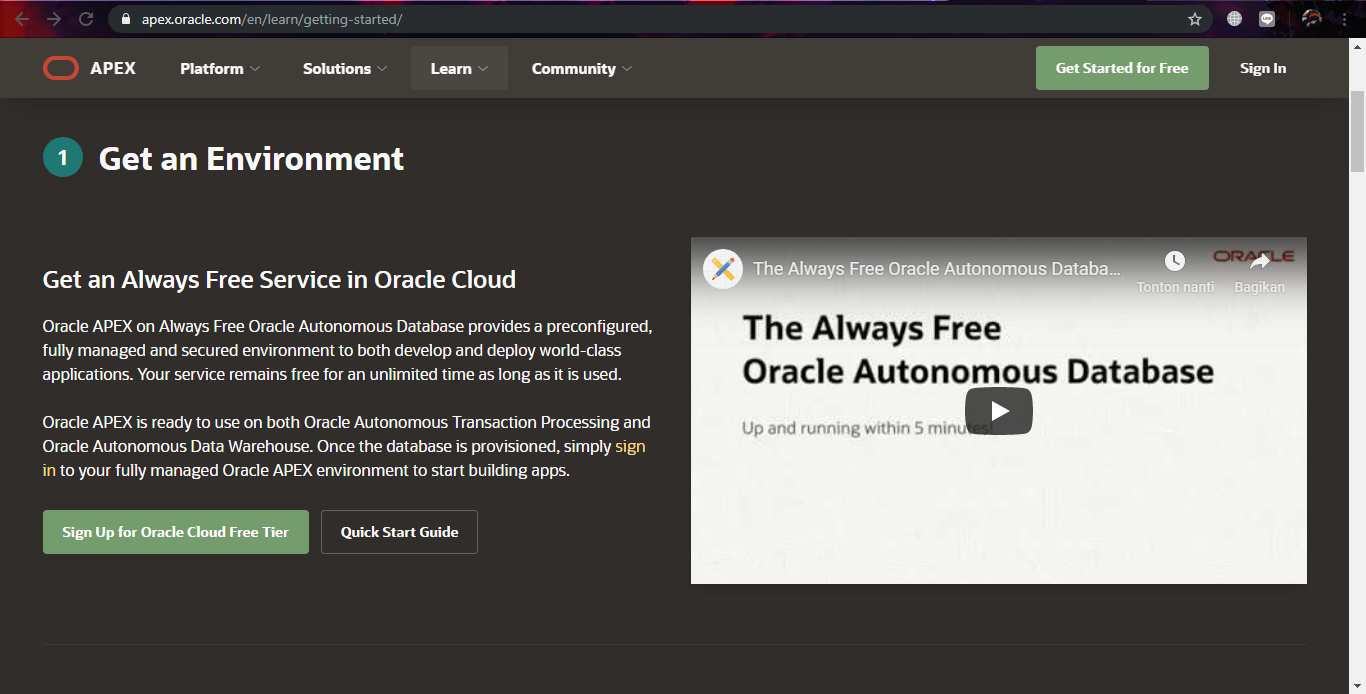
\includegraphics[scale=0.3]{figure/1.PNG}
        \caption{Halaman Awal}
    \end{figure}
    \item Jika sudah maka langsung klik bagian \textit{request free workspace}
\newpage
    \item Jika sudah, maka akan masuk ke laman ini.
    \begin{figure}[!htbp]
        \centering
        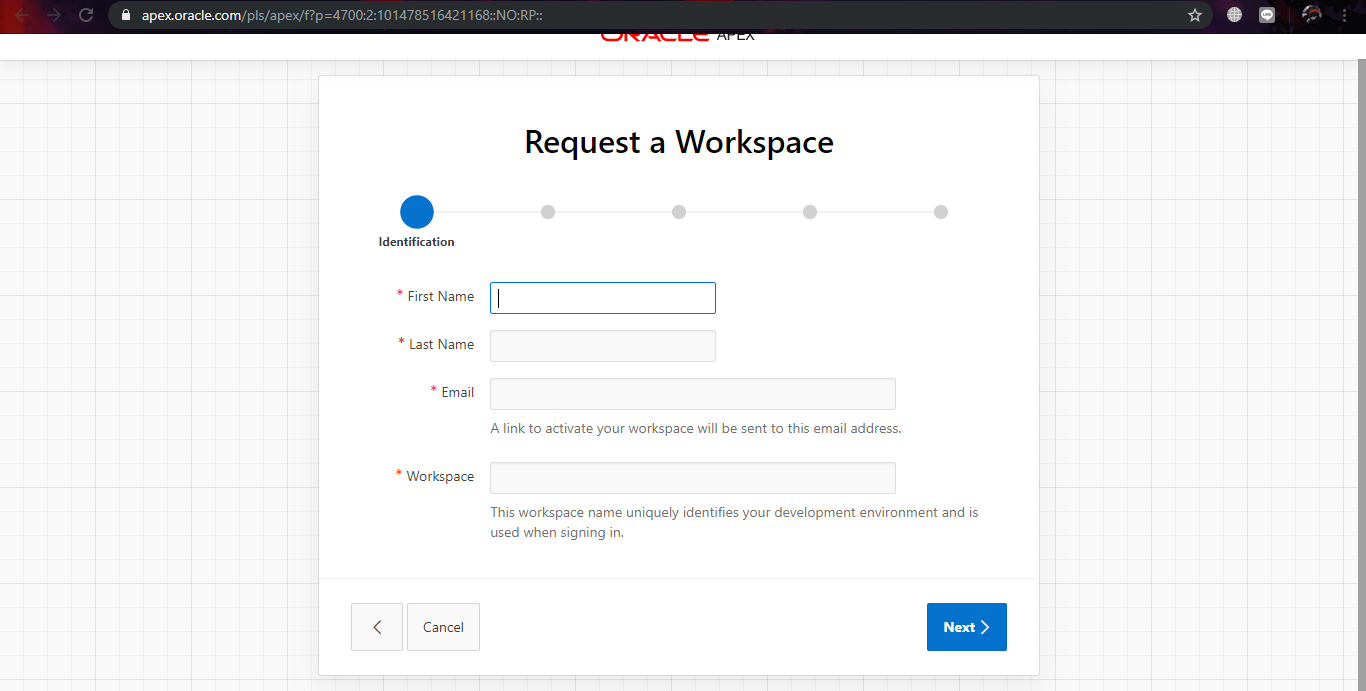
\includegraphics[scale=0.3]{figure/2.PNG}
        \caption{Konfigurasi Workspace}
    \end{figure}
    \item Selanjutnya masukkan firstname, lastname dan yang lainnya sesuai dengan keinginan anda
    \item Jika sudah, langsung lanjut dan masuk ke halaman ini.
    \begin{figure}[!htbp]
        \centering
        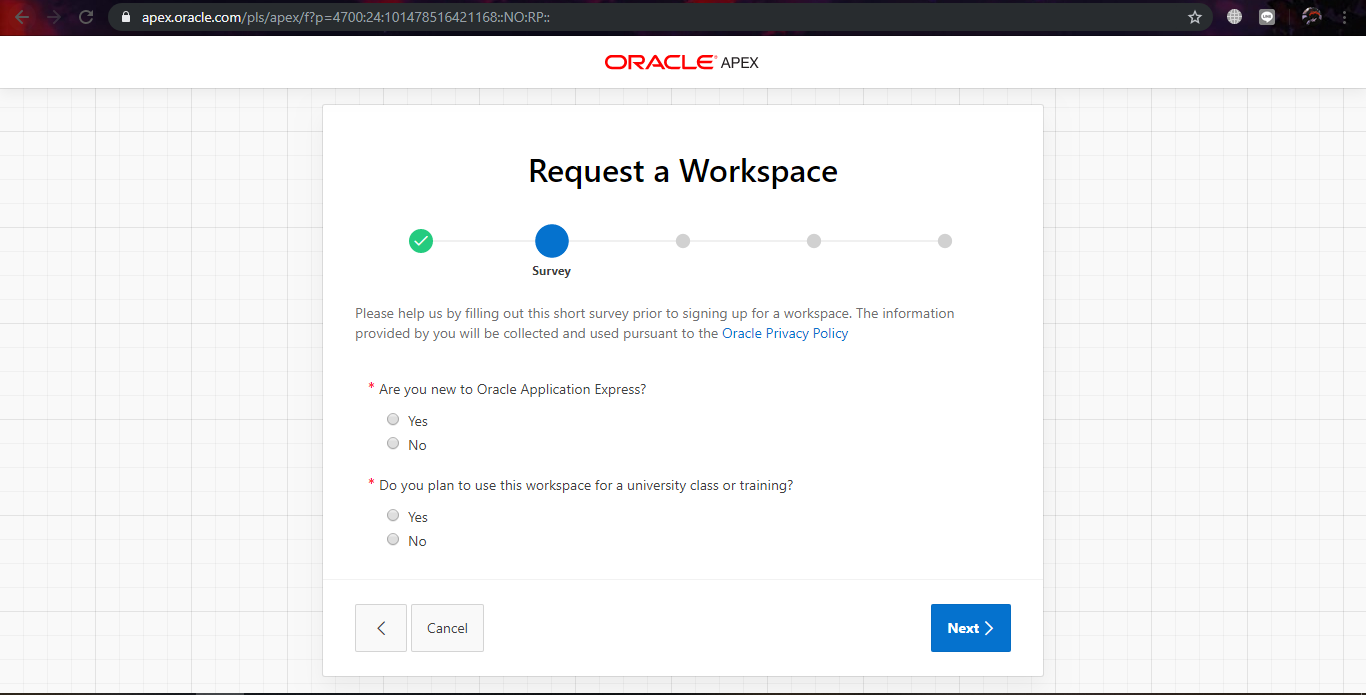
\includegraphics[scale=0.3]{figure/3.PNG}
        \caption{Konfigursi Workspace(2)}
    \end{figure}
\newpage
    \item Pilih sesuai dengan keinginan anda.
    \item Selanjutnya klik next dan akan muncul tampilan seperti ini.
    \begin{figure}[!htbp]
        \centering
        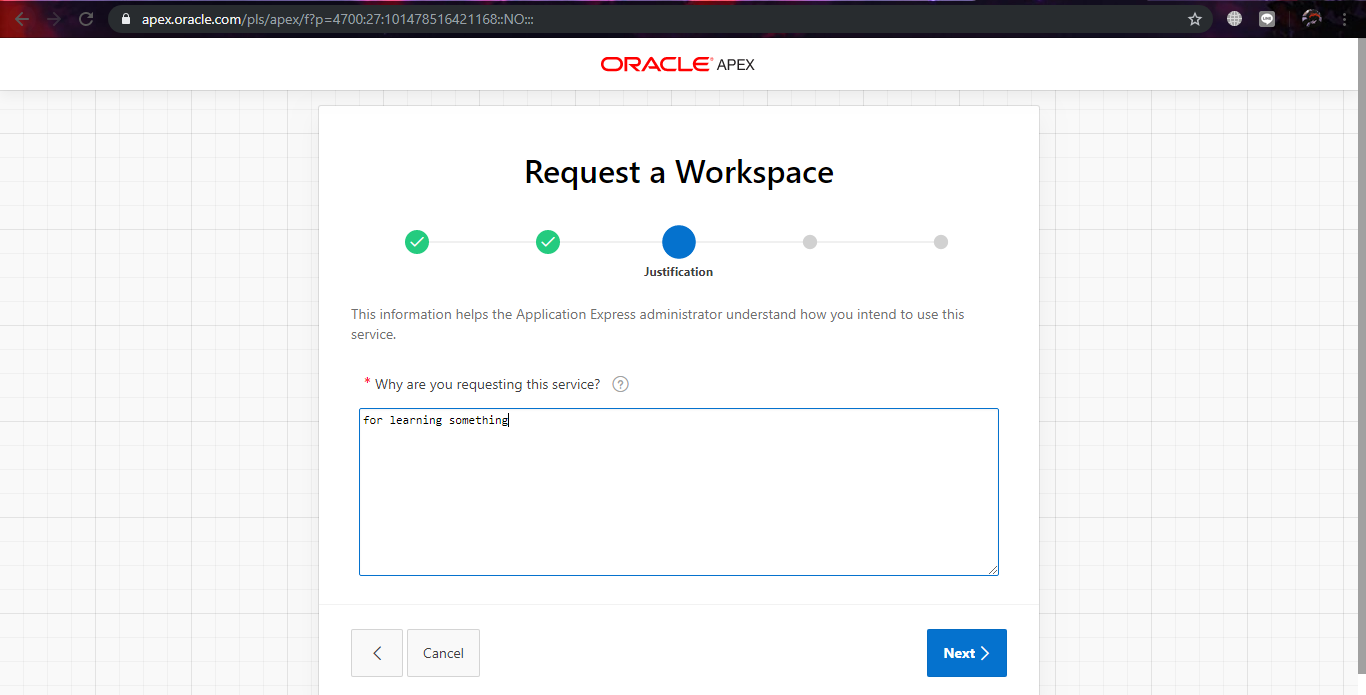
\includegraphics[scale=0.3]{figure/4.PNG}
        \caption{Konfigurasi Workspace(3)}
    \end{figure}
    \item Isi sesuai keinginan kalian.
    \item Setelah itu klik next dan akan muncul tampilan seperti ini.
    \begin{figure}[!htbp]
        \centering
        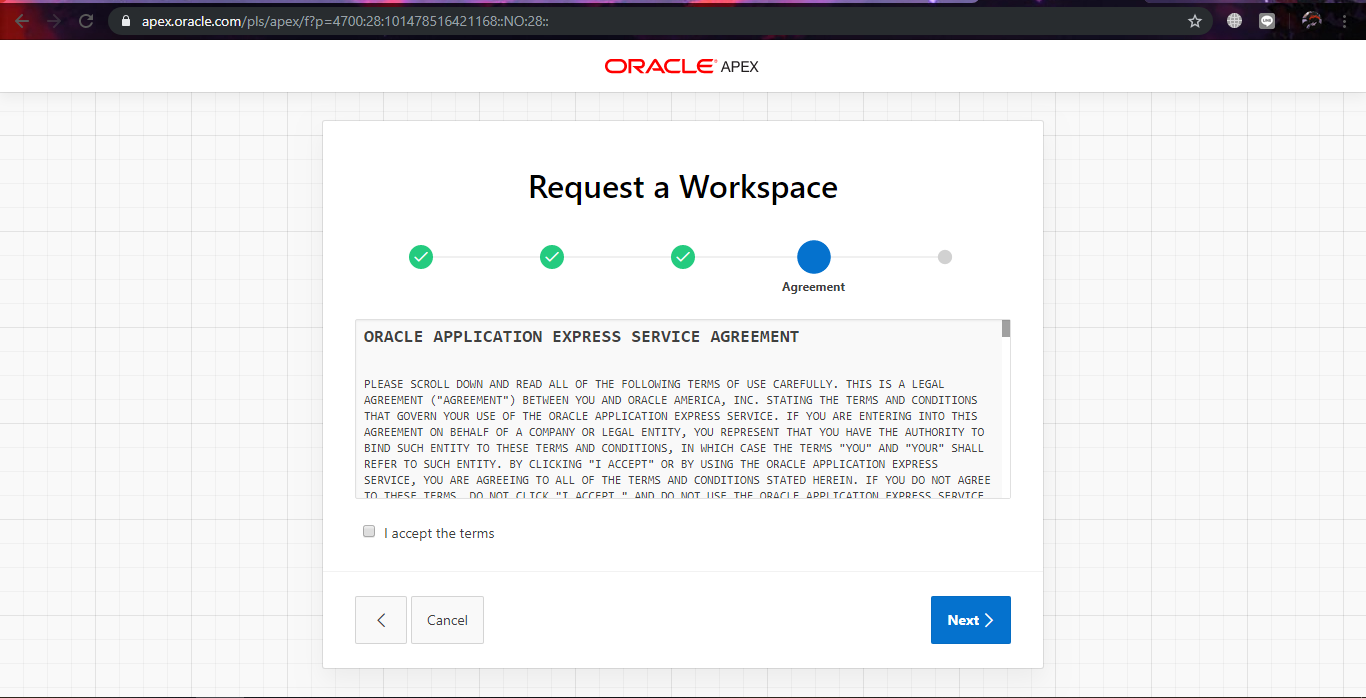
\includegraphics[scale=0.3]{figure/5.PNG}
        \caption{Konfigurasi Workspace(4)}
    \end{figure}
\newpage
    \item Klik accept, dan next
    \item Seterusnya klik submit dan request dan akan muncul tampilan seperti ini
    \begin{figure}[!htbp]
        \centering
        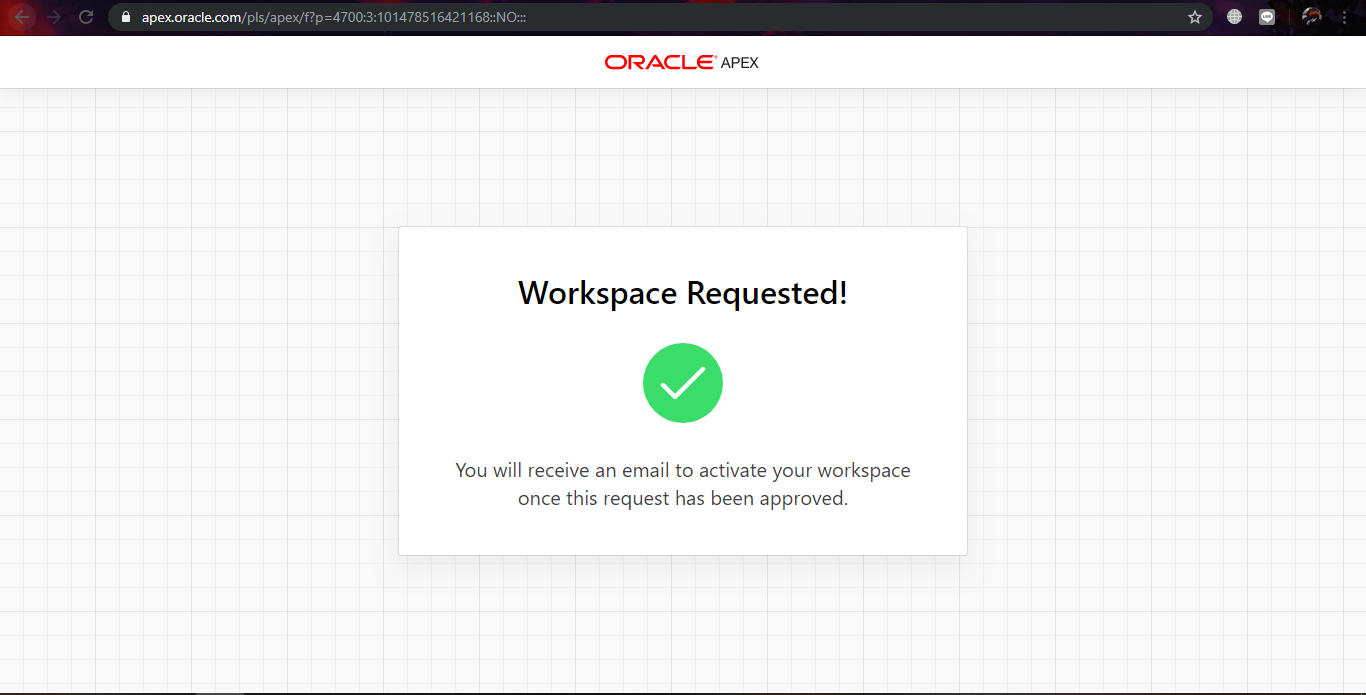
\includegraphics[scale=0.3]{figure/6.PNG}
        \caption{Konfigurasi Workspace(5)}
    \end{figure}
    \item Kalian tinggal ngecek email dan mengaktifkan workspace tersebut
    \item Jika sudah di klik pada bagian email kalian, maka akan muncul pemberitahuan \textit{workspace successfully created}
    \begin{figure}[!htbp]
        \centering
        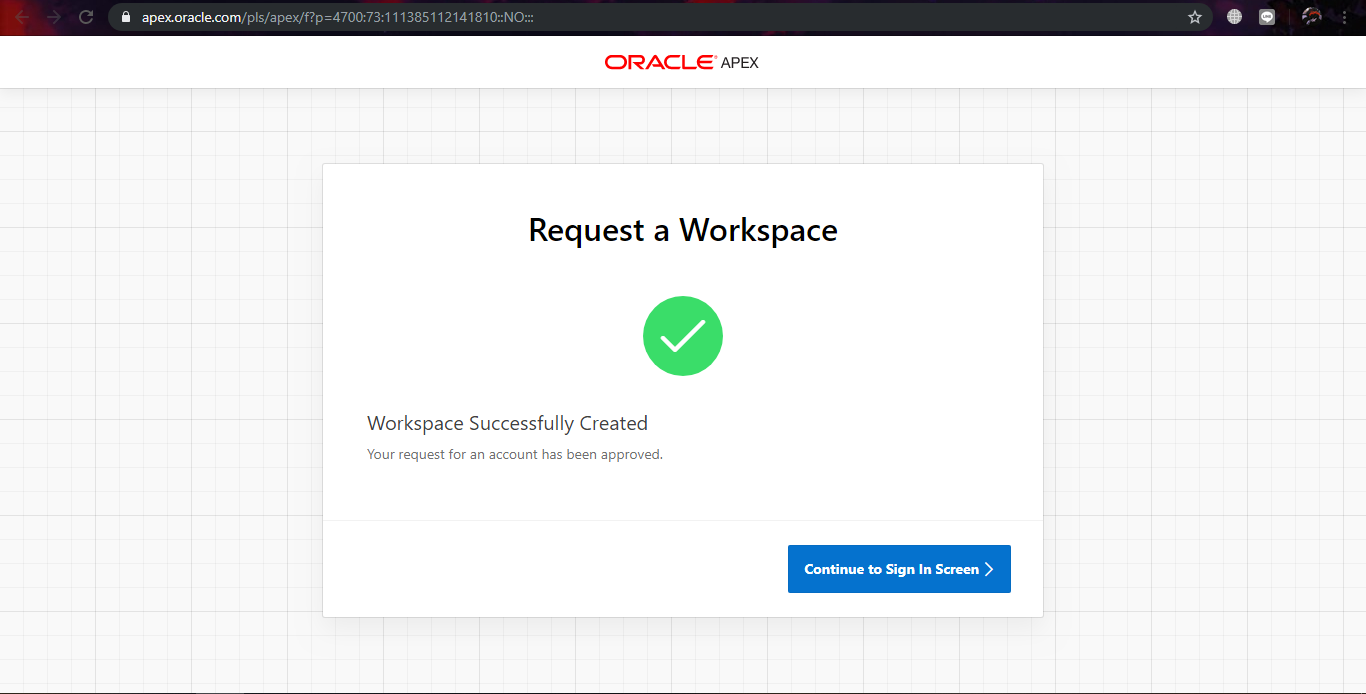
\includegraphics[scale=0.3]{figure/7.PNG}
        \caption{Workspace telah dibuat}
    \end{figure}
\end{enumerate}
\newpage
\section{Membuat Aplikasi}
\paragraph{}
Sebelum membuat aplikasi, pastikan anda sudah membuat data nya terlebih dahulu pada \textit{Microsoft Excel} seperti contoh dibawah ini.
\begin{figure}[!htbp]
    \centering
    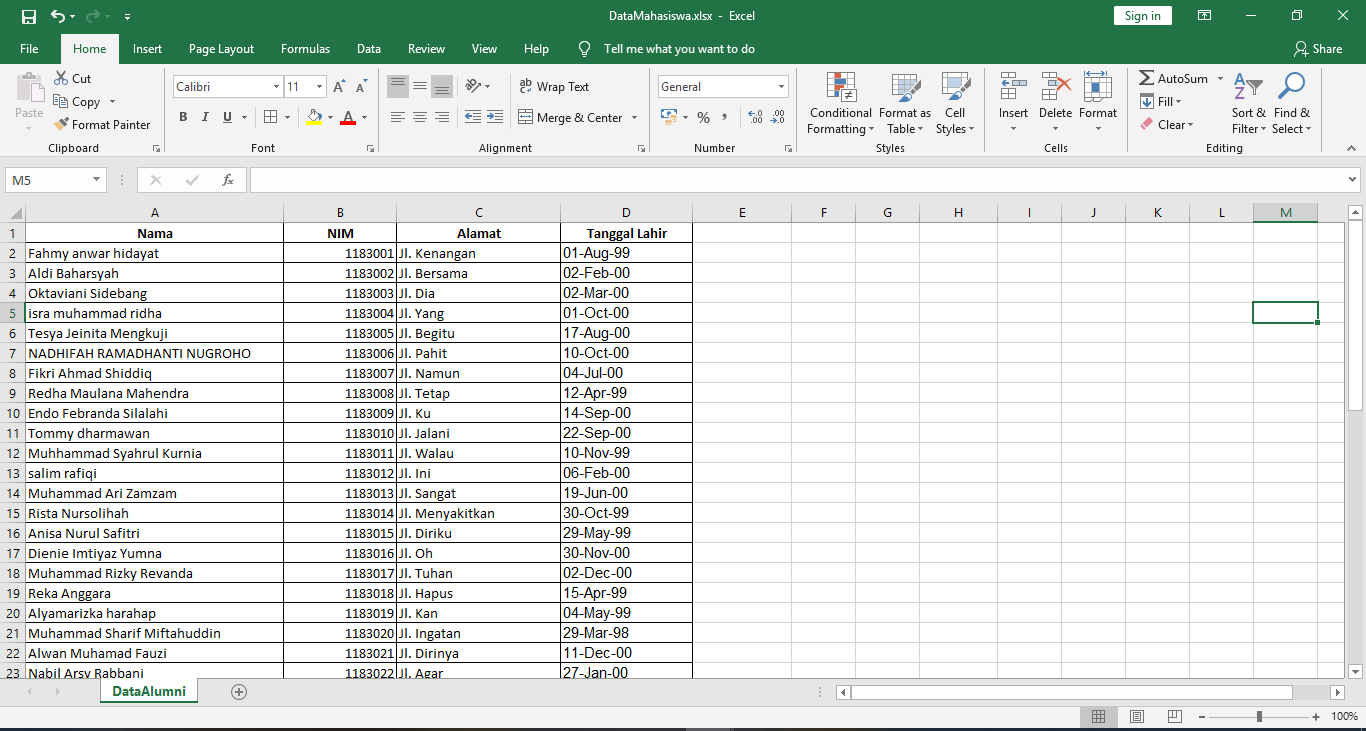
\includegraphics[scale=0.3]{figure/Data.PNG}
    \caption{Data Mahasiswa}
\end{figure}
    \subsection{Langkah-langkah}
    \begin{enumerate}
        \item Pertama, kalian akan login terlebih dahulu ketika sudah selesai membuat 
    \begin{figure}[!htbp]
        \centering
        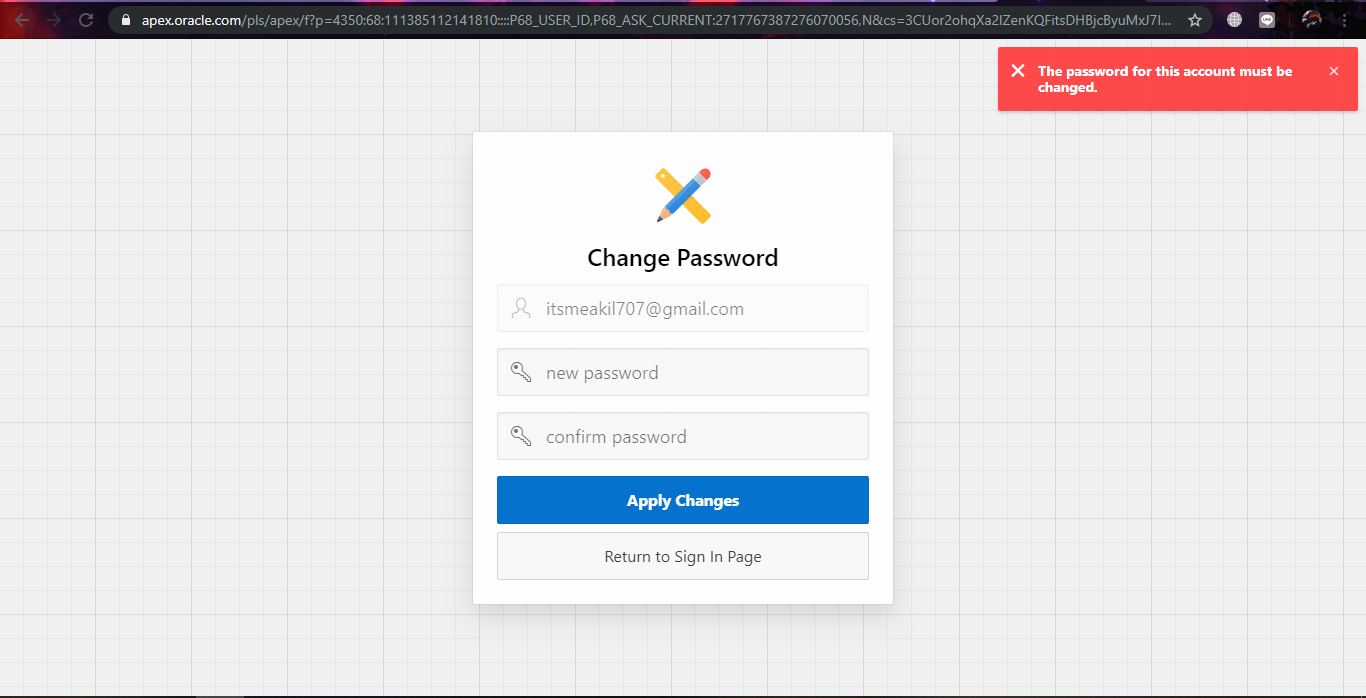
\includegraphics[scale=0.3]{figure/8.PNG}
        \caption{Login}
    \end{figure}
    \item Ada pemberitahuan bahwa password harus diubah, maka password kalian ubah.
\newpage
    \item Selanjutnya klik next maka akan masuk ke halaman utama apex.
    \begin{figure}[!htbp]
        \centering
        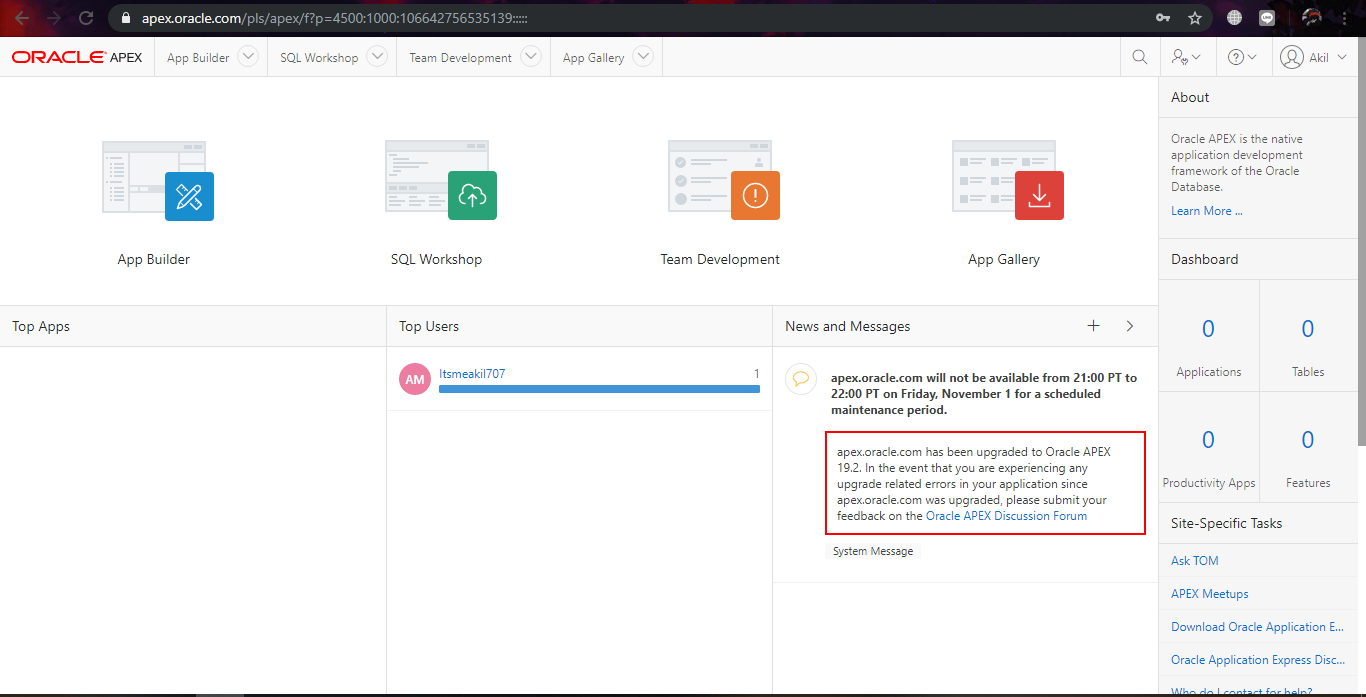
\includegraphics[scale=0.3]{figure/9.PNG}
        \caption{Halaman Utama}
    \end{figure}
    \item Setelah itu, klik bagian \textit{App Builder}
    \item Dan akan ada tampilan seperti ini
    \begin{figure}[!htbp]
        \centering
        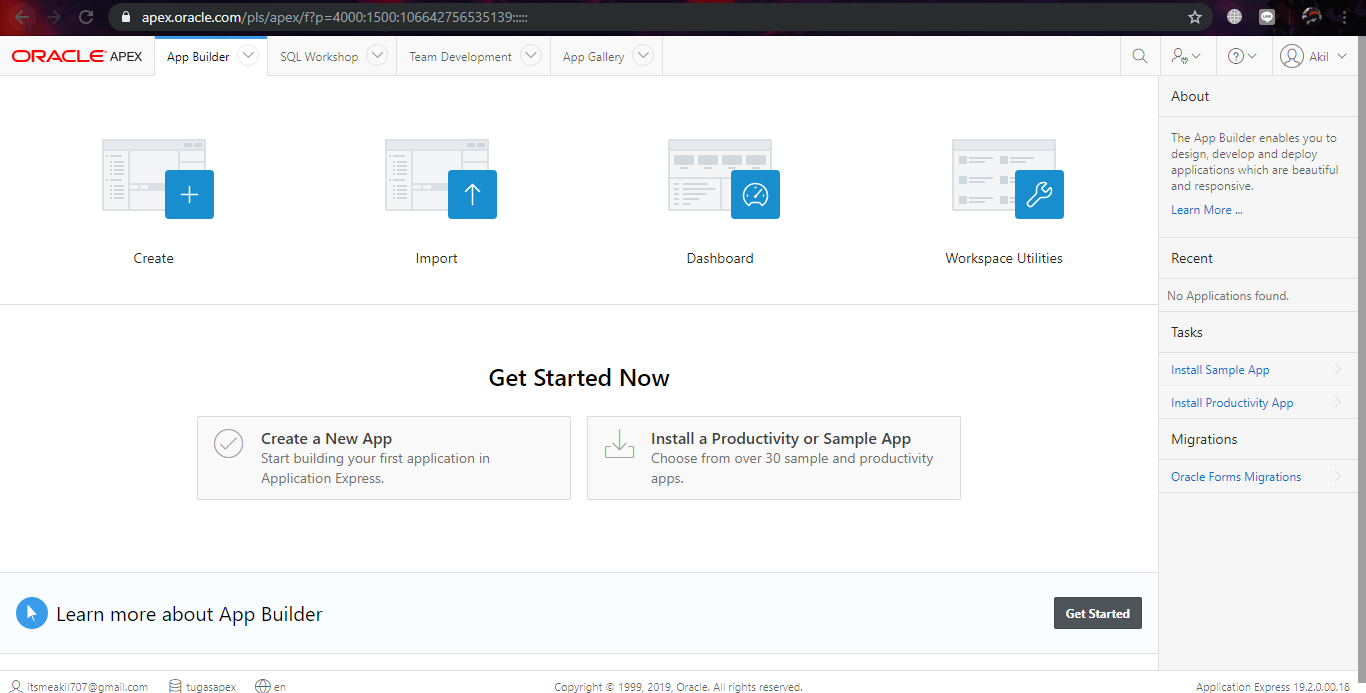
\includegraphics[scale=0.3]{figure/10.PNG}
        \caption{Halaman App Builder}
    \end{figure}
    \item Setelah itu klik create dan akan ada tampilan seperti ini
    \begin{figure}[!htbp]
        \centering
        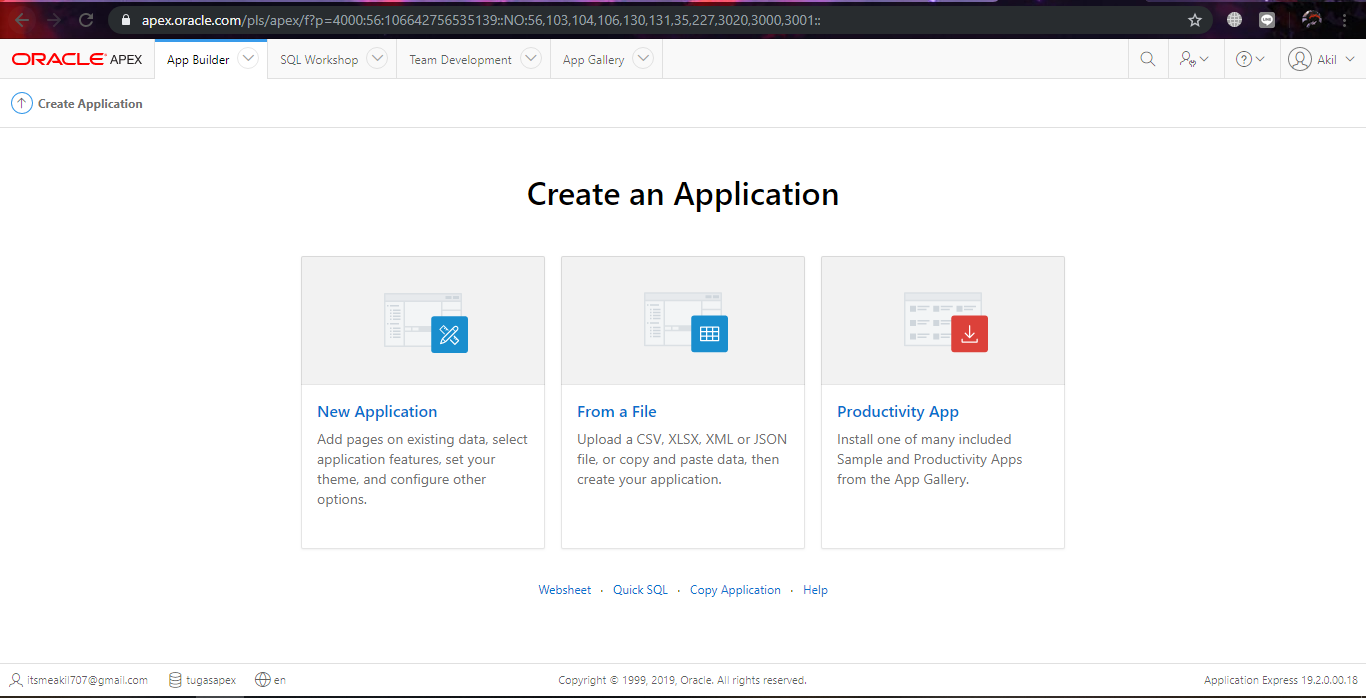
\includegraphics[scale=0.3]{figure/11.PNG}
        \caption{Create Application}
    \end{figure}
\newpage
    \item Pilih upload file
    \item Dan pilih file csv yang sudah kita sediakan
    \begin{figure}[!htbp]
        \centering
        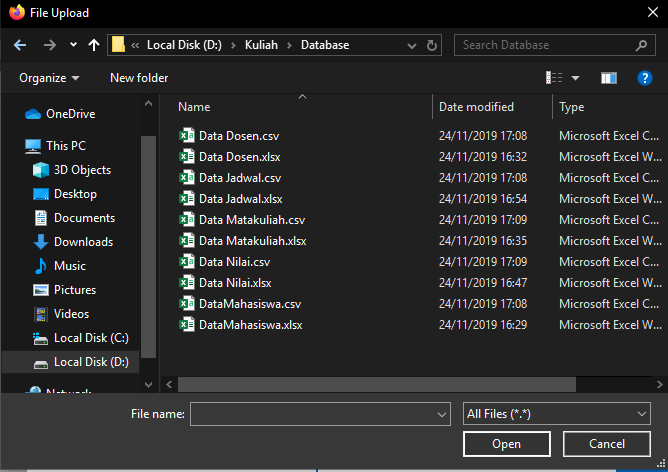
\includegraphics[scale=0.6]{figure/csv.PNG}
        \caption{Data yang akan di upload}
    \end{figure}
\newpage
    \item Jika sudah, maka lakukan seperti dibawah ini
    \begin{figure}[!htbp]
        \centering
        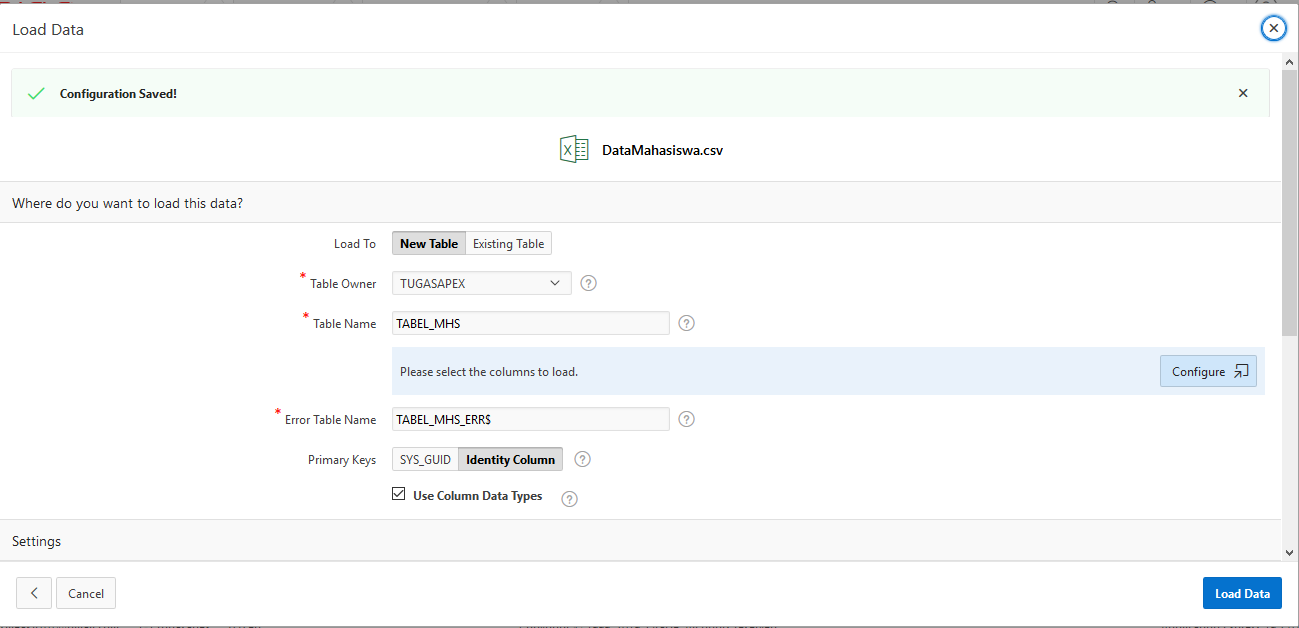
\includegraphics[scale=0.3]{figure/load.PNG}
        \caption{Caption}
    \end{figure}
    \item Jika selesai, maka tinggal load data, dan berhasil
    \begin{figure}[!htbp]
        \centering
        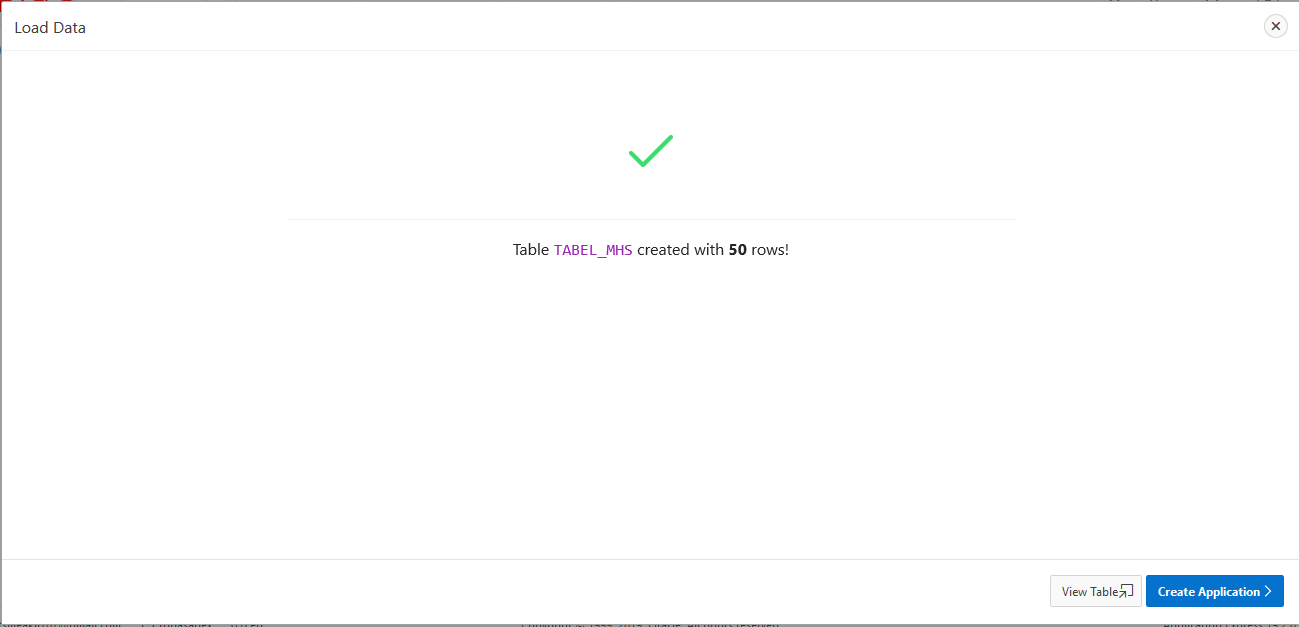
\includegraphics[scale=0.3]{figure/loadberhasil.PNG}
        \caption{Load Berhasil}
    \end{figure}
    \item Lakukan hal tersebut berulang-ulang sebanyak data yang kamu upload.
\newpage
    \item Jika sudah maka tinggal create application
    \item Langkah Selanjutnya ialah relasi tabel tersebut
    \item Pertama drop semua id yang ada pada semua tabel
    \item Pilih bagian drop column, dan pilih id
    \begin{figure}[!htbp]
        \centering
        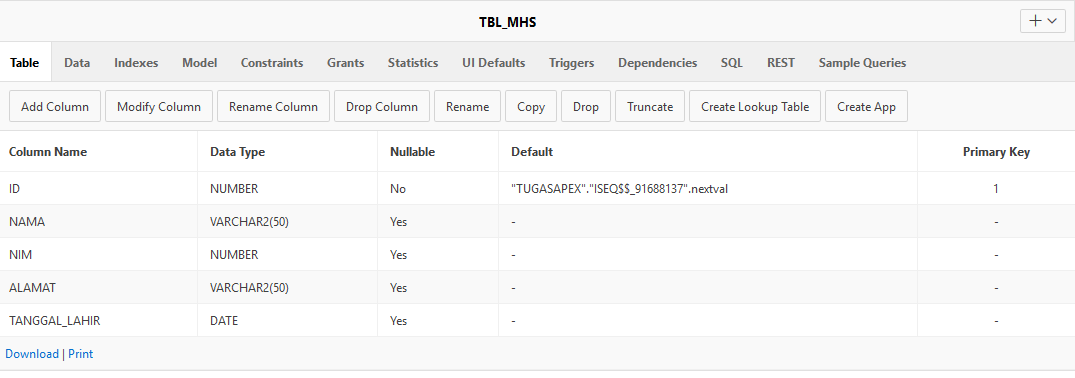
\includegraphics[scale=0.4]{figure/dropid.PNG}
        \caption{Drop ID}
    \end{figure}
    \item Lakukan ini ke semua tabel
    \item Jika sudah, maka lakukan perintah untuk menentukan primary key.Primary key diambil dari suatu yang unique yang tidak dapat disamakan.
    \begin{figure}[!htbp]
        \centering
        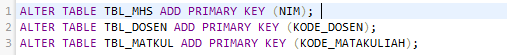
\includegraphics[scale=0.8]{figure/primarykey.PNG}
        \caption{Perintah Primary Key}
    \end{figure}
    \item Jika sudah maka langkah selanjutnya menentukan foreign key untuk bisa direlasikan
    \item Perintah nya ialah seperti ini
    \begin{figure}[!htbp]
        \centering
        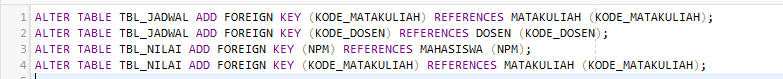
\includegraphics[scale=0.5]{figure/foreignkey.PNG}
        \caption{Perintah Foreign Key}
    \end{figure}
\newpage
    \item Data yang dibuat sudah selesai, sekarang kembali ke halaman utama
    \item Dan klik create
    \item Setelah create, kita akan klik bagian new application
    \begin{figure}[!htbp]
        \centering
        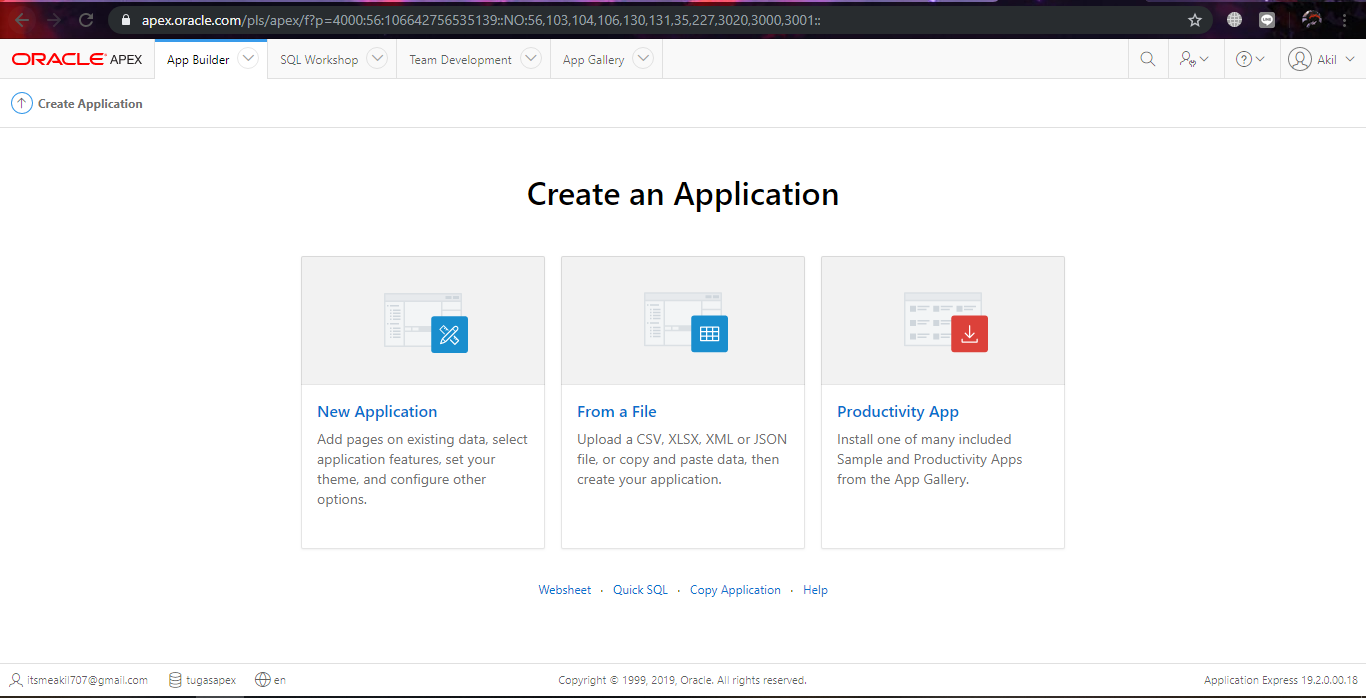
\includegraphics[scale=0.3]{figure/11.PNG}
        \caption{Klik Create Application}
    \end{figure}
    \item Jika sudah maka, beri nama apl yang kalian inginkan
    \item Setelah itu, klik add page
    \begin{figure}[!htbp]
        \centering
        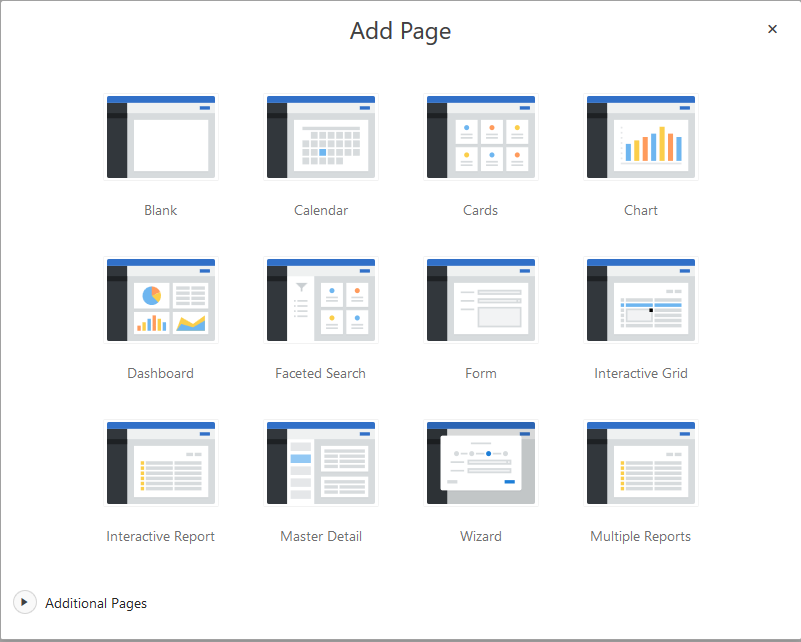
\includegraphics[scale=0.4]{figure/addpage.PNG}
        \caption{Add Page}
    \end{figure}
\newpage
    \item Pilih interactive report
    \item Jika sudah, maka akan seperti ini
    \begin{figure}[!htbp]
        \centering
        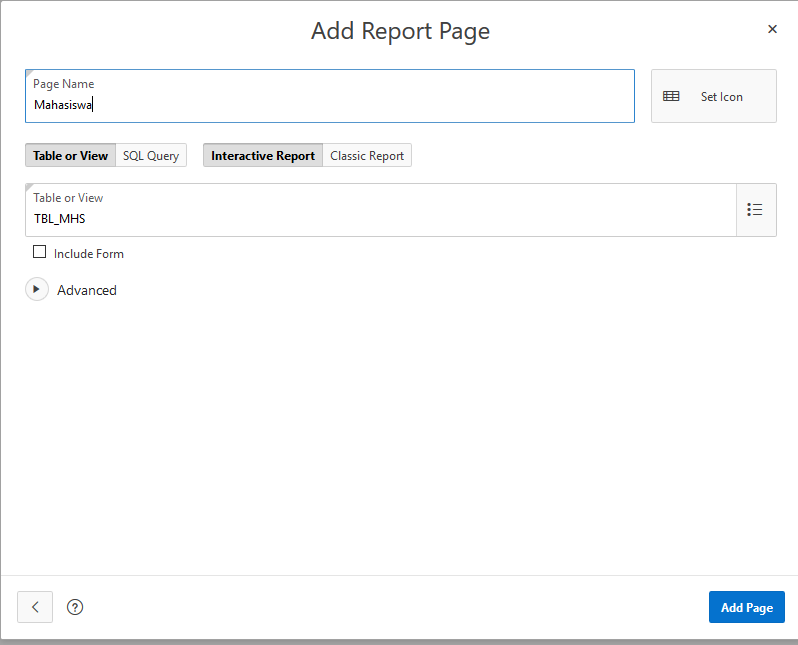
\includegraphics[scale=0.4]{figure/createpage.PNG}
        \caption{Create Page}
    \end{figure}
    \item Pilih nama page sesuai yang diinginkan
    \item Pilih tabel yang ingin ditampilkan
    \item Jika sudah maka add page
    \item Lakukan hal yang sama ke page lain seperti matakuliah dan dosen.
\newpage
    \item Jika sudah semua, maka selanjutnya ke jadwal dan nilai.
    \item Lakukan perintah add page, tapi tidak memilih tabel, melainkan melakukan query seperti dibawah
    \begin{figure}[!htbp]
        \centering
        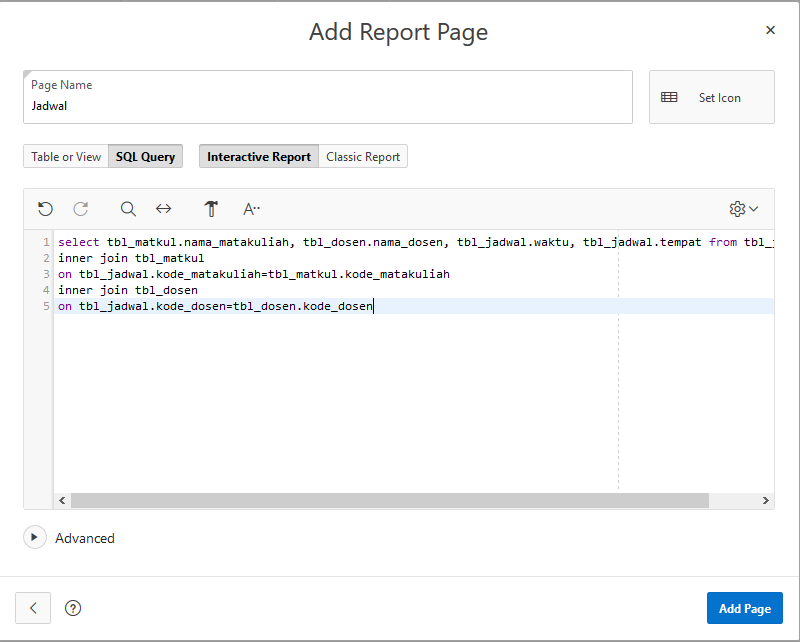
\includegraphics[scale=0.4]{figure/innerjoinjadwal.PNG}
        \caption{Inner Join Jadwal}
    \end{figure}
    \item Lakukan query diatas, dan save
    \item Lakukan perintah yang sama untuk nilai
    \item Jika sudah maka tinggal kita create application
\newpage
    \item Ketika di run, maka akan ada hal login
    \begin{figure}[!htbp]
        \centering
        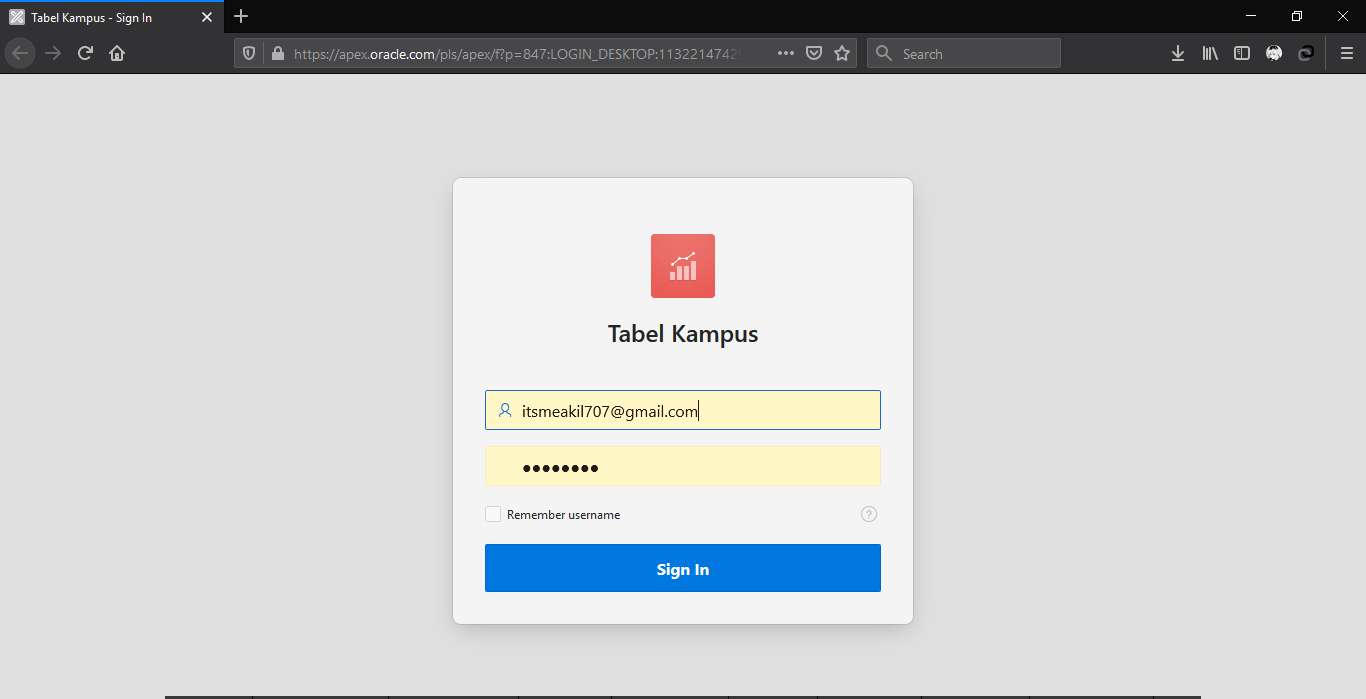
\includegraphics[scale=0.3]{figure/login.PNG}
        \caption{Login ke aplikasi}
    \end{figure}
    \item Berikut username dan pass nya
    \begin{figure}[!htbp]
        \centering
        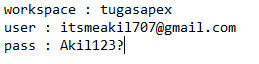
\includegraphics{figure/userapex.PNG}
        \caption{username dan pass}
    \end{figure}
\newpage
    \item Jika sudah maka tampilan aplikasi nya akan seperti ini
    \begin{figure}[!htbp]
        \centering
        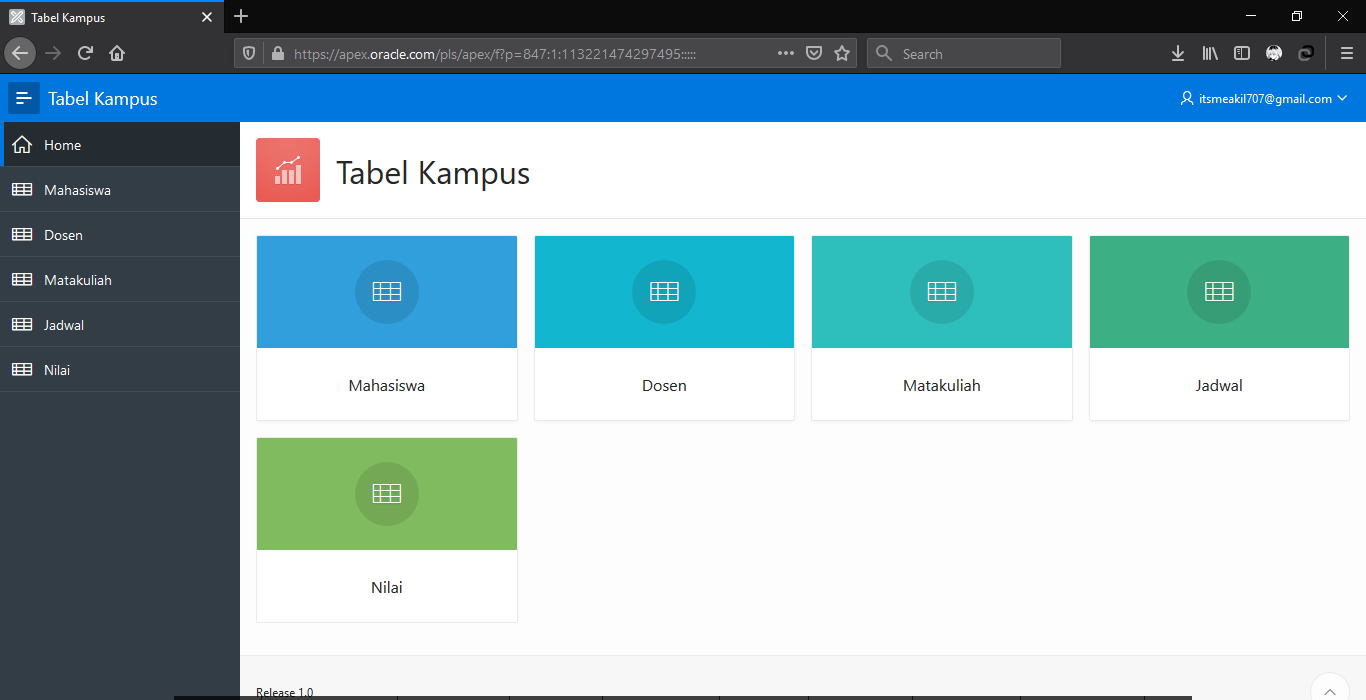
\includegraphics[scale=0.3]{figure/apl.PNG}
        \caption{Aplikasi}
    \end{figure}
    \item Aplikasi sudah jadi :D
    \end{enumerate}
\end{document}